\documentclass[twoside,a4paper,12pt]{uathesis}
\usepackage[percent]{overpic}
\usepackage{algorithm}
\usepackage{algorithmic}

\renewcommand{\algorithmicrequire}{\textbf{Input:}}
\renewcommand{\algorithmicensure}{\textbf{Output:}}

%make fonts searchable
%\usepackage{cmap}
%\input{glyphtounicode}
%\pdfgentounicode=1


\usepackage[T1]{fontenc}
\usepackage{lmodern}
\usepackage{amsmath}
%\usepackage{amsfonts}
\usepackage{amsthm}
\usepackage{graphicx}
\usepackage[export]{adjustbox}
\usepackage{url} % format email, hypertext, and path addresses
%\usepackage[figure,linesnumbered,commentsnumbered,shortend,noline]{algorithm2e}
\usepackage{subfigure}
\usepackage{xspace}

\usepackage{fancyvrb}
%\usepackage{bera} %for bold in verbatim 
%\usepackage{amsmath}
\usepackage{bm}

\usepackage[format=plain,labelfont=up]{caption}
\usepackage{multirow}
\usepackage{xcolor}
\usepackage{colortbl}
%\usepackage[export]{adjustbox} %used to adjust trim image
\usepackage{afterpage}
\usepackage{booktabs} %for tables to use functions such as \toprule
\usepackage{comment}

\usepackage{enumitem} %used to change enum and list spaces and settings

\usepackage{listings}
\lstset{
%     language=C,
    captionpos=b,
    breaklines=true,
%     frame=single,
    basicstyle=\footnotesize,
    numbers=left,
    numberstyle=\bf\scriptsize,
    stepnumber=1,
    numbersep=5pt,
    escapeinside={(*@}{@*)}
%     emph={solution},emphstyle={\color{red}},
%     emph={[2]phOut,oxygenOut,waterOut},emphstyle={[2]\color{blue}},
%     emph={[3]sensors,operatorStop},emphstyle={[3]\color{Green}}
}
\lstdefinelanguage{Esterel}{
    morekeywords={abort, and, await, call, case, combine, constant do, each,
                  else, elsif, emit, end, every, exec, exit, false, function,
                  halt, handle, if, immediate, in, input, inputoutput, loop,
                  mod, module, not, nothing, or,output, pause, positive, pre,
                  present, procedure, relation, repeat, return, run, sensor,
                  signal, suspend, sustain, task, then, tick, timeout, times,
                  trap, true, type, upto, var, watching, weak, when, with
                 },
    sensitive=true,
    morecomment=[l]{\%},
    morestring=[b]",
}

\usepackage{hyperref}
\hypersetup{
    pdfauthor={Keyan Monadjem},
    hidelinks
}
\usepackage{bookmark}

\newbox\subfigbox
\makeatletter
\newenvironment{subfloat}
{\def\caption##1{\gdef\subcapsave{\relax##1}}
  \let\subcapsave\@empty
  \setbox\subfigbox\hbox
  \bgroup}
{\egroup
  \subfigure[\subcapsave]{\box\subfigbox}}
\makeatother

%\newcommand{\comment}[1]{{}}
\newcommand{\dontprintsemicolon}{\DontPrintSemicolon}


\newtheorem{definition}{Definition}
%\newtheorem{proof}{Proof}
\newtheorem{theorem}{Theorem}

\newenvironment{abbreviations}{%
    \if@twocolumn
      \@restonecoltrue\onecolumn
    \else
      \@restonecolfalse
    \fi
    \chapter*{List of \abbreviationsname}%
      \@mkboth{\abbreviationsname}%
              {\abbreviationsname}%
  }
  {\newpage\@mkboth{}{}}
\newcommand\abbreviationsname{Abbreviations}

\begin{document}

\title{Safe Synchronous Artificial Neural Networks}
\author{Keyan Themba Monadjem}
\department{Electrical \& Computer Engineering}
\submitdate{February 2019}
\supervisor[Dr. Partha S. Roop]

%create the title page
\maketitle

%%%%%%%%%%%%% First section %%%%%%%%%%%%%%%
\frontmatter
\bookmark[page=3]{Abstract}
\include{Abstract}

\bookmark[page=5]{Acknowledgements}
\include{Acknowledgements}

%create table of contents
\bookmark[page=7]{Contents} % Sets a PDF bookmark for the contents page
\tableofcontents

\bookmark[page=11]{List of Figures}
\listoffigures

\bookmark[page=15]{List of Tables}
\listoftables

%\cleardoublepage
%\phantomsection
%\addcontentsline{toc}{chapter}{List of Abbreviations}
%\input{abbreviations}

%%%%%%%%%%%% Body of the Thesis %%%%%%%%%%%
\mainmatter

%\include{Introduction/Introduction}
\chapter{Test Chapter}

Hello World

%\include{LiteratureReview/LiteratureReview}

%\include{Background/Backgound}

%\include{Semantics/Semantics}
%
%\include{PRET/PRET}
%

%
%\{Compilation/Compilation}
%
%\include{TimingAnalysis/TimingAnalysis}

%\include{Results/Results}

\chapter{Run-time Verification}

\section{Methodology} 
The system designed for this case study was made to reflect a \acf{AV} and its object detection mechanisms. 
The system used multiple techniques to tackle the inherent issues of the \ac{AV} system, i.e. weakness to perturbed inputs and misclassification detection.
The system's sensors include an overhead, 360$^\circ$ \acf{LiDAR} apparatus, and a single, frontal facing camera.
A solitary camera was sufficient to prove the efficacy of this solution, however it is to be noted that \ac{AV} systems generally use multiple cameras, facing different directions, so that the controller can make properly informed decisions.
The system used can be seen in Figure~\ref{fig:ssnn}. 

The \ac{LiDAR} for this system was accurate 93\% of the time~\cite{lidarFusion}, to closely simulate a real \ac{LiDAR} system.
The simulated camera outputs consisted of test images from both the \ac{VOC}~\cite{pascal-voc-2012} and \ac{GTSRB}~\cite{Stallkamp2012-gtsrb} datasets, in a combination of people, vehicles and various traffic signs.
The \ac{LiDAR} and camera outputs were handled by different parts of the controller.
The camera outputs were fed into a \ac{MNN} (see Figure~\ref{fig:mnn}) where they were classified by shape, colour and object type.

Utilising synchronous semantics, a \acf{MNN}, containing three other \ac{MNN} ensembles, was created.
Each ensemble synchronously combined the outputs of three different convolutional \acfp{SNN}~\cite{sann}, providing increased prediction accuracy for shape, colour and object type. 
These ensembles ran in synchronous concurrency, each taking four logical ticks to run. 
The outputs of each ensemble were then combined into batch of outputs forming the \textit{predicted output}. 

The system controller was encapsulated by a run-time enforcer~\cite{recps} that used sensor fusion to check for misclassifications made by the \ac{MNN}.
A safety automata (timed automata)~\ref{?} was designed to verify predictions made by the \ac{MNN} and ensure utmost safety at all times.
The automata started in a safe state, where control of the vehicle was autonomously handled by the system controller.
If a misclassification was detected, the enforced policy entered an unstable state, still under autonomous control. 
Once enough time passed without further misclassifications, the vehicle entered the safe state again.
However, if another misclassification was detected while unstable, the enforced policy entered a violation state and forced control of the \ac{AV} to the driver.
The vehicle would not enter autonomous mode again until the system was restarted.
A diagram of the enforced policy's safety (timed) automaton is shown in Figure~\ref{fig:signrte}.
This type of run-time enforcement, where neither the inputs nor outputs of the sensors or controller are enforced, has been termed as \textit{run-time verification}.
\textit{Run-time verification} refers to the verification of system parameters during run-time, while ensuring that the system is aware of any failed guards in the enforced policy.


\begin{figure}[t]
	\centering
	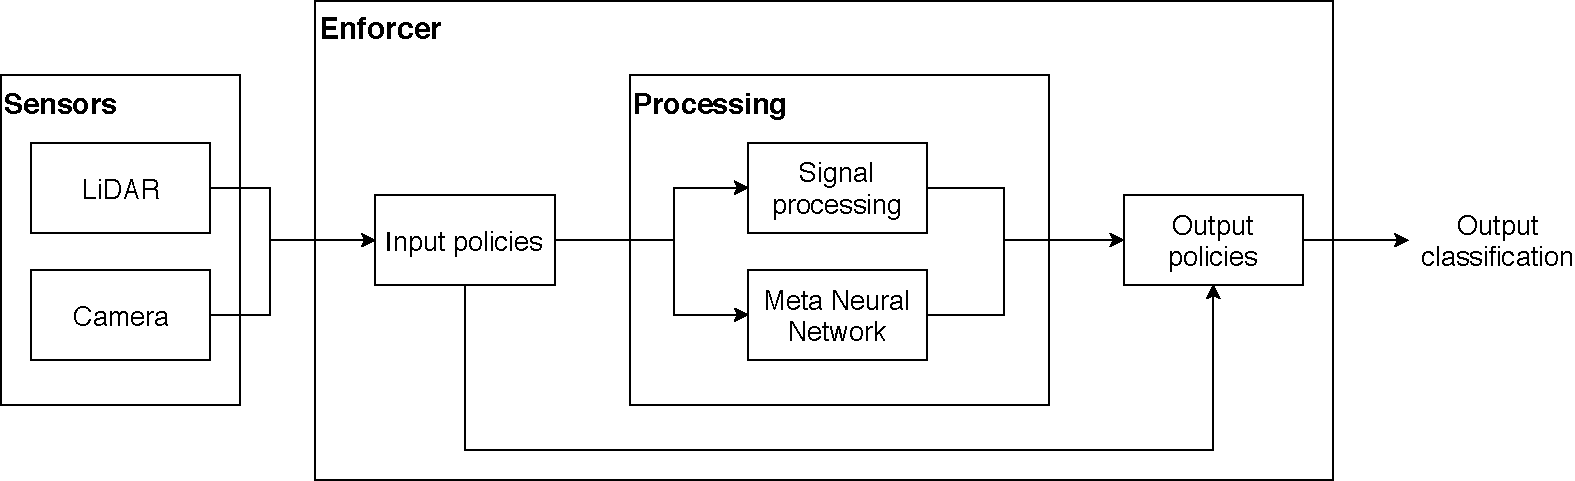
\includegraphics[scale=0.6]{Content/fig/SSNN.pdf}
	\caption{Block diagram showing the AV system with enforcer}
	\label{fig:ssnn}
\end{figure}

\begin{figure}[h]
	\centering
	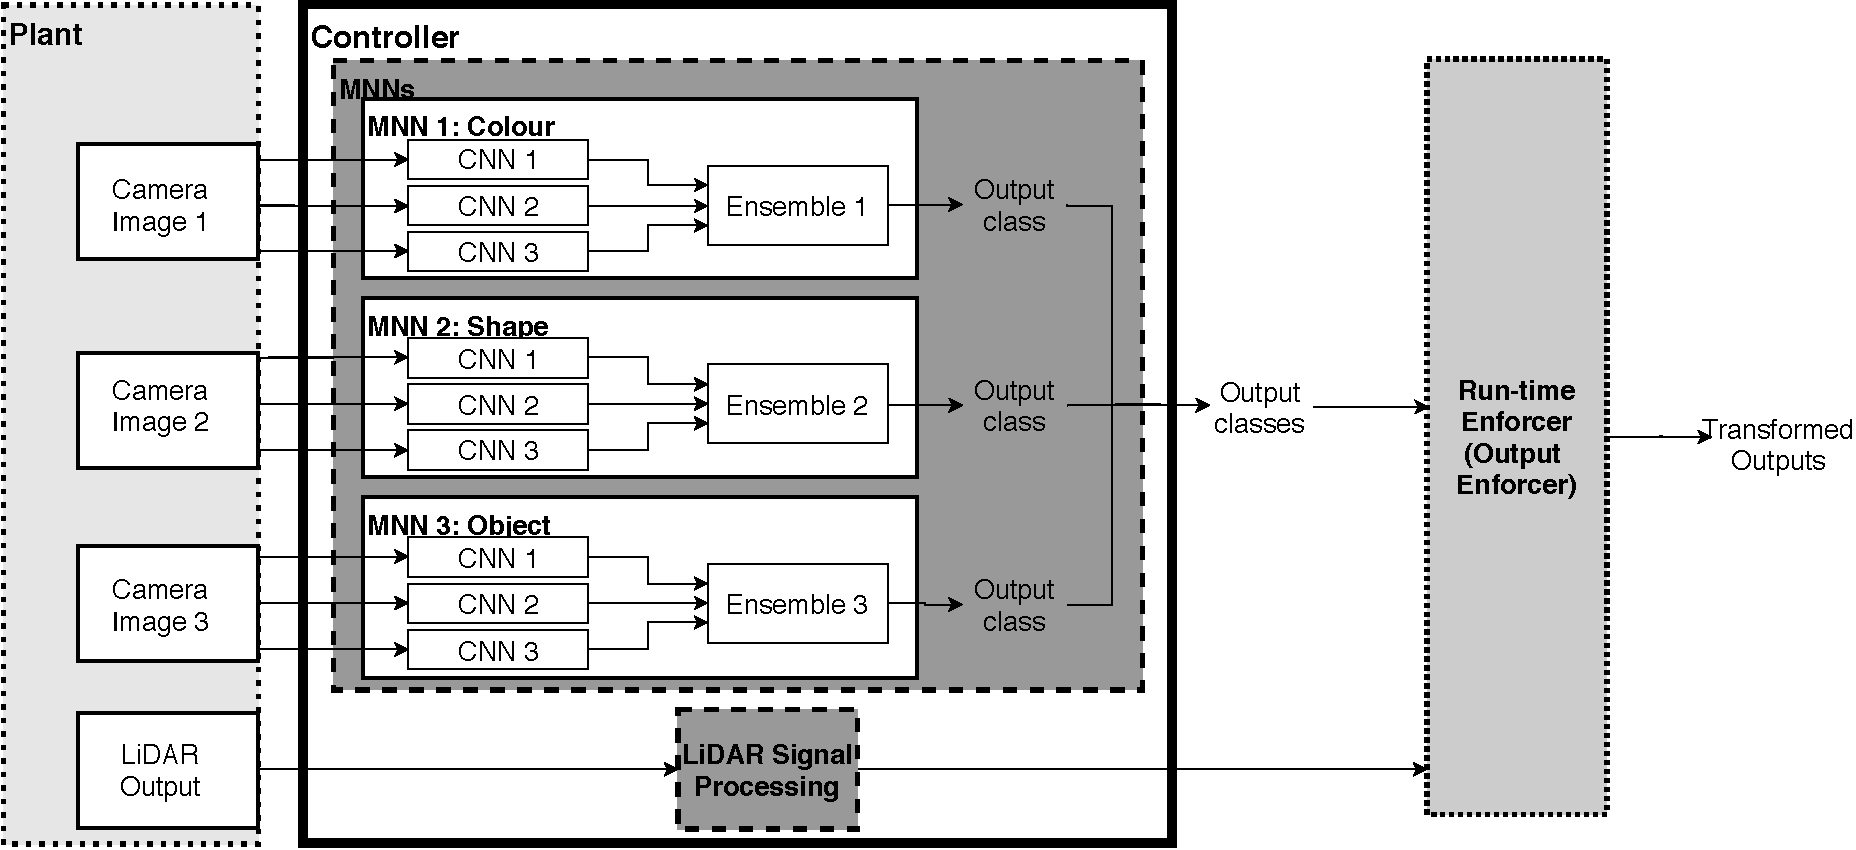
\includegraphics[scale=0.9]{Content/fig/MNN.pdf}
	\caption{Block diagram showing the Meta Neural Network ensemble} \label{fig:mnn}
\end{figure}

\begin{figure}[t]
	\centering
	\scalebox{1.3}{

\begin{tikzpicture}[>=stealth',shorten >=1pt,auto,node distance=3 cm, scale = 1, transform shape]

\tikzstyle{accept} = [draw=blue!75,fill=blue!20]
\tikzstyle{violate} = [draw=red!75,fill=red!40, dashed]
\tikzstyle{unstable} = [draw=red!75,fill=red!15]

\node[initial,state, accepting, accept] (A) {$q_{auto}$};
\node[state, unstable] (B) [right of=A] {$q_{unstable}$};
\node[state, violate]         (C) [below of=B, xshift=-1.5cm]  {$q_v$};

\path[->] 
		(A) edge [loop above]       node [above]  
		{
			\scriptsize$\let\scriptstyle\textstyle\substack{\overline{M}}$
		} (A)
		
		(A) edge [bend left]		node [below]  
		{
			\scriptsize$\let\scriptstyle\textstyle\substack{
				M,~\\~
				t~:=~0~
			}$
		} (B)
	
		(B) edge [loop above]		node [above]  
		{
			\scriptsize$\let\scriptstyle\textstyle\substack{t~<~3~\&~\\~~\overline{M}}$
		} (B)
	
		(B) edge [bend left]		node [right]  
		{
			\scriptsize$\let\scriptstyle\textstyle\substack{M}$
		} (C)
	
		(B) edge [bend left]		node [below]  
		{
			\scriptsize$\let\scriptstyle\textstyle\substack{t~>=~3~\&\\~\overline{M}}$
		} (A)
	
		(C) edge [loop below] node [below]
		{
			\scriptsize$\sum$
		}(C)
		;

\end{tikzpicture}}

	\begin{itemize}
		\item $P$: Misclassification of a person.
		\item $V$: Misclassification of a vehicle.
		\item $N$: Classification of an object when there is nothing.
		\item $S$: Misclassification of a traffic sign.
		\item $C$: Confidence rating of the \ac{SNN} classification.
		\item $t$: Timer for the unstable state.
	\end{itemize}
	
	\caption{Enforcer policy for the AV prediction system}
	\label{fig:signrte}
\end{figure}




















\begin{comment}
\include{temp}
\end{comment}





\include{Conclusions/Conclusions}

\appendix
\chapter{Appendix}


%\include{Publications}


%%%%%%%%%%%% Last part of thesis indices, bibliography  %%%%%%%%%%%%
\backmatter

%create the bibliography
% \bibliographystyle{siam}
\renewcommand{\bibname}{References}
% \clearpage
\phantomsection
\addcontentsline{toc}{chapter}{\bibname}
\bibliographystyle{IEEEtranS}
\bibliography{references}


\end{document}

